\section{Durchführung}
\label{sec:Durchführung}

\subsection{Versuchsaufbau}
\label{sec:Versuchsaufbau}

Der schematische Versuchsaufbau besteht zum einen aus einer Spule in die eine Probe 
eingeführt 
werden kann und zum anderen aus zwei Polschuhen, die in ihrem Zwischenraum ein 
äußeres Magnetfeld erzeugen können, inwelchem sich die eben genannte Spule befindet. 
Das durch die Polschuhe erzeugte Magnetfeld entspricht $\vec{B}_{\text{0}}$.
In der Spule selbst wird das Hochfrequenzfeld $\vec{B}_{\text{1}}$ erzeugt.
An die Spule ist ein Empfänger angeschlossen, der in der Lage ist, das Induktionssignal 
welches durch die Präzession der Magnetisierung hervorgerufen wird, zu messen.
Das empfangene Signal kann daraufhin auf einem Oszilloskop sichtbar gemacht werden.
%Der reale Versuchsaufbau wurde mit einer Teachspin-Apparatur \ref{fig1} 
%durchgeführt.
%\begin{figure}
%  \centering
% 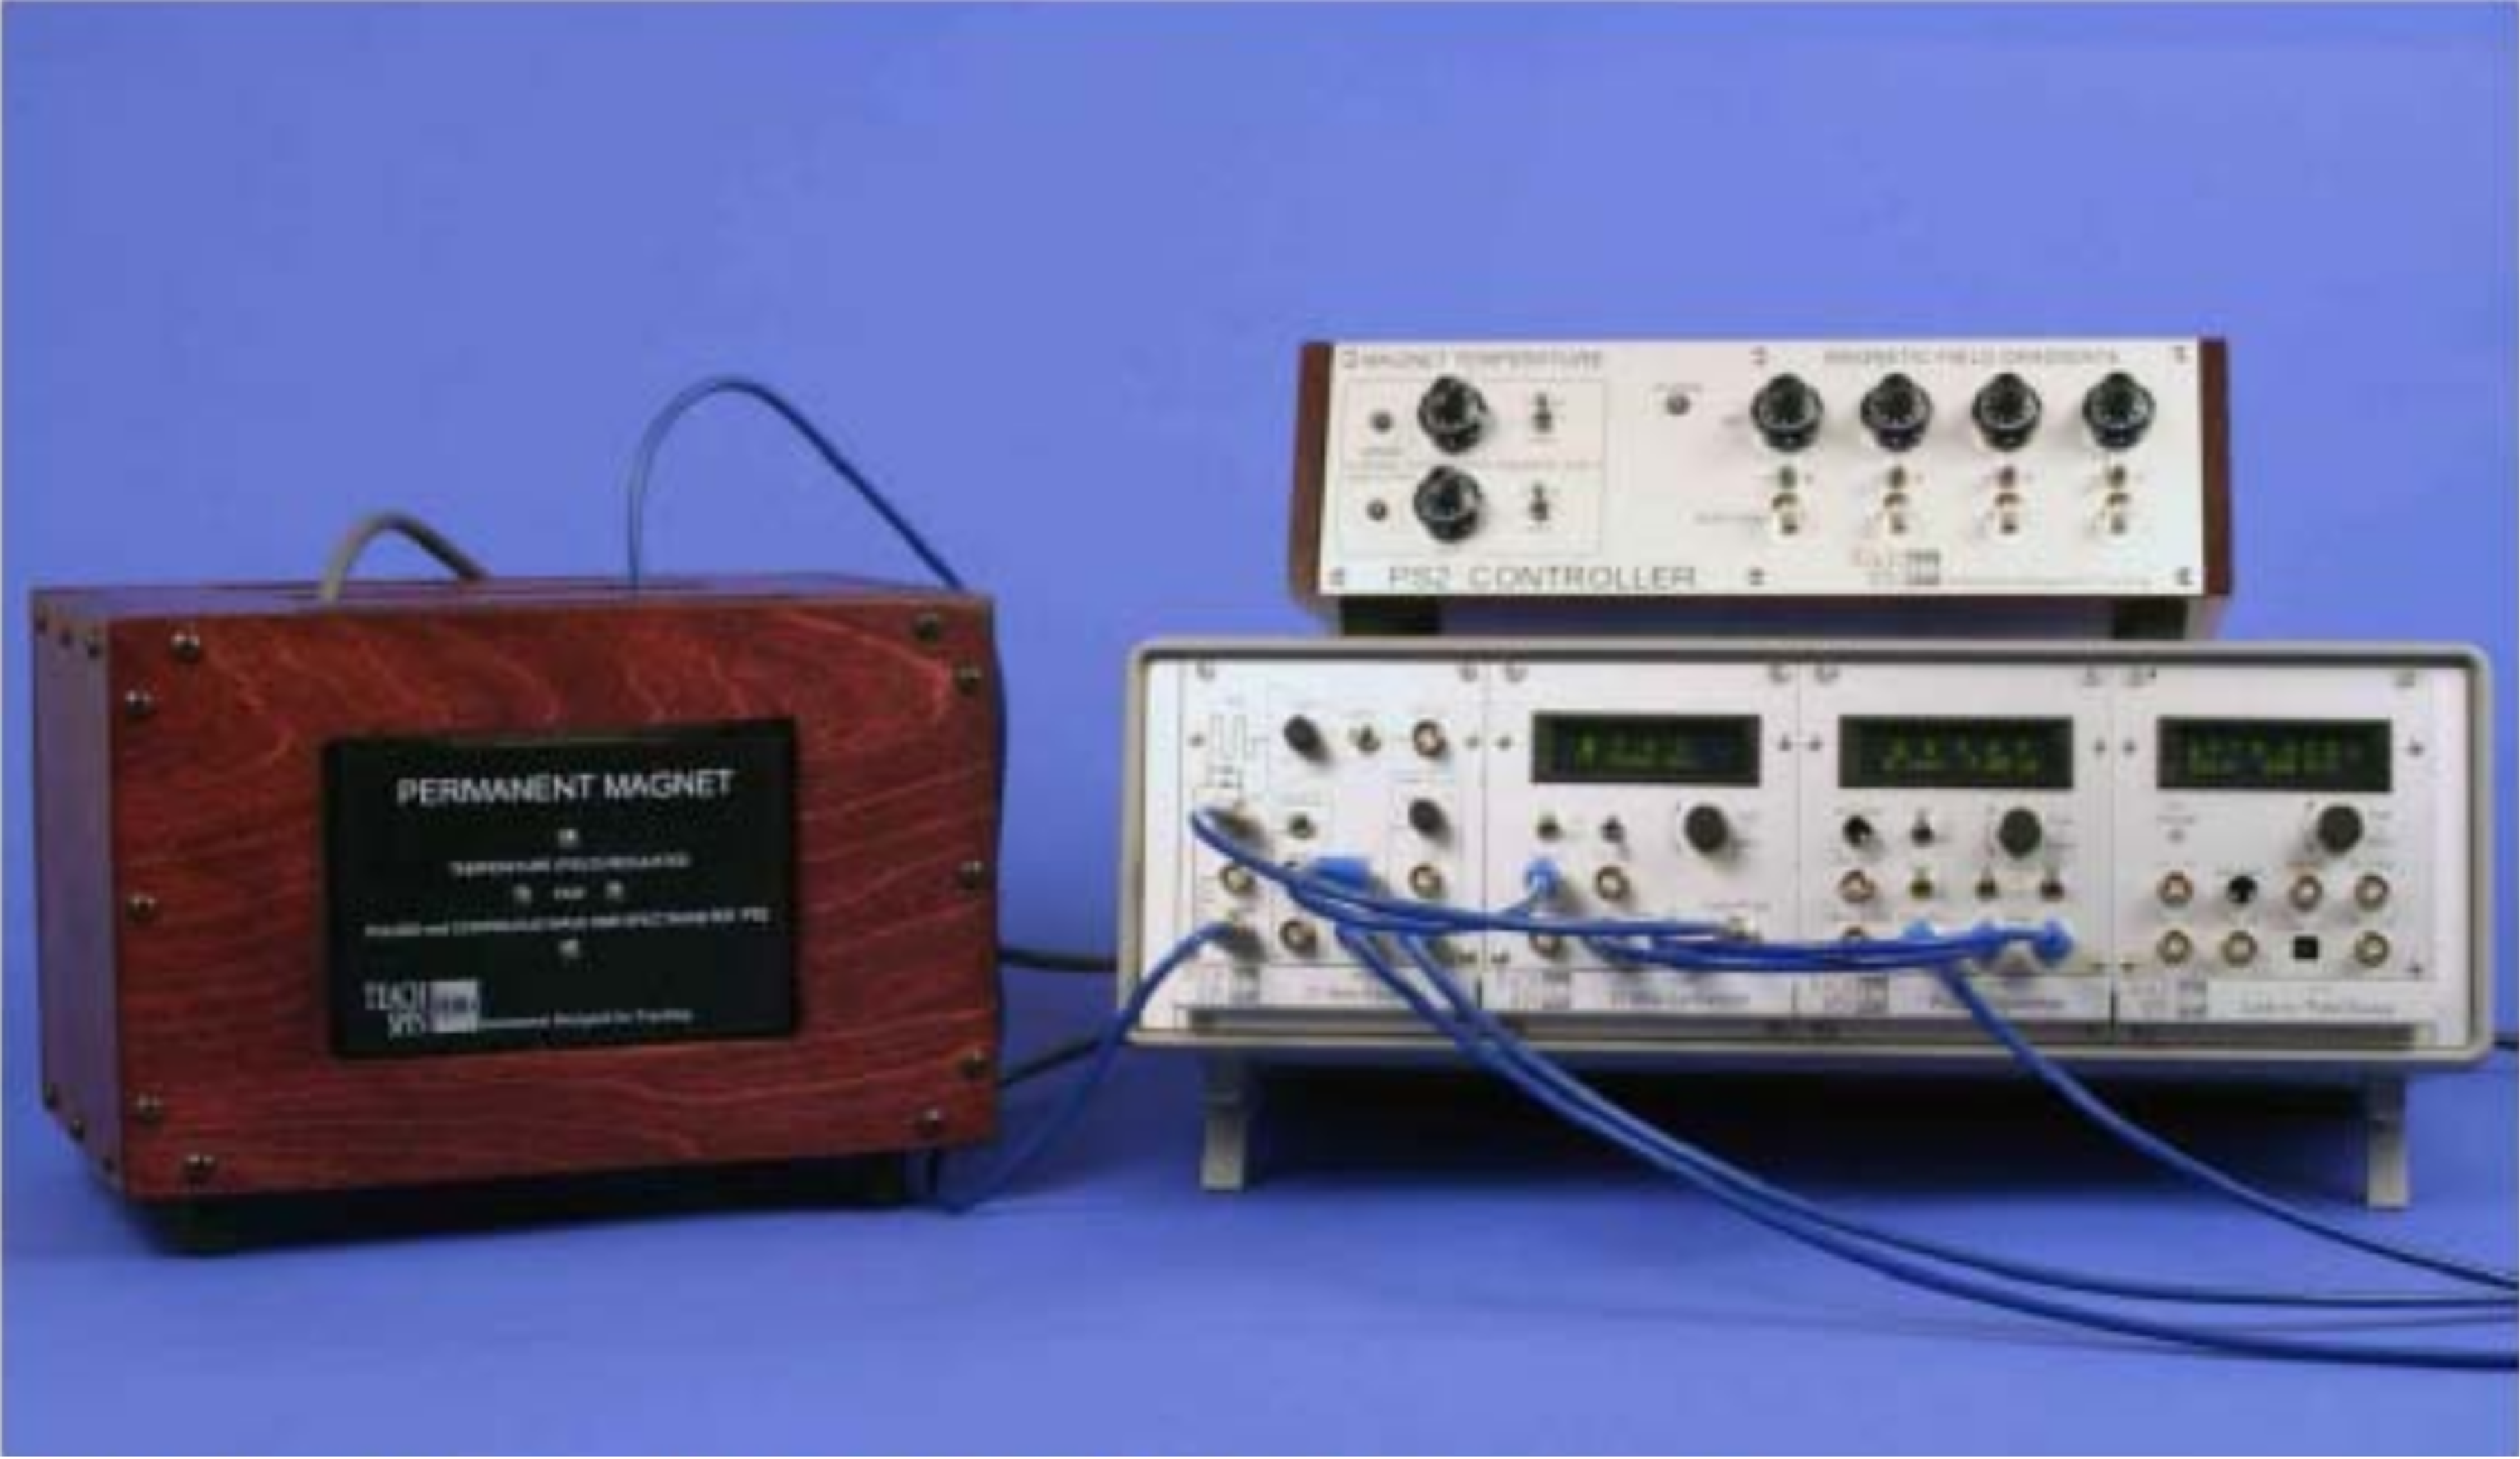
\includegraphics[width=.7\textwidth]{images/teachspin.pdf}
%  \caption{Links im Bild sind die Polschuhe um die Spule verbaut, während
%  die Einstellungen der Messungsparamter an der Apparatur rechts vorgnommen 
% werden können \cite{anleitung}.}
%  \label{fig1}
%\end{figure}

\subsection{Justage und Temperaturmessung}
\label{sec:Justage}

Zum justieren wird anstelle einer reinen Wasserprobe eine mit Kupfersulfat 
durchsetzte Probe verwendet. Diese Alternative führt zu verkürztenn Relaxationszeiten.
Zunächst werden die Gradientenspulen auf die Werte
\begin{align}
    x = -1.0\\
    y = -5.0\\
    z = 3.7\\
    z^2 = -2.4
\end{align}
eingestellt. Bei diesen Werten wird das Magnetfeld so homogen wie möglich.
Die Frequenz wird auf $\SI{21,71585}{\mega\hertz}$ eingestellt,
da bei diesem Wert die Signalschwingungen am geringsten sind. Die Phase wird auf 
-130° eingestellt, sodass fast nur Signal im Realteil erscheint.
Da sich die Pulslängen zwischen dem ersten Puls A und dem zweiten Puls B 
um den Faktor 2 unterscheiden müssen (siehe Abblidung \ref{fig}) wird A auf 
$\SI{2,7}{\micro\second}$ und B auf $\SI{5}{\micro\second}$ eingestellt.
